\subsection{Обзор инструментов}
\label{subsections:Tools}

\paragraph{Unity}

В качестве фреймворка для выполнения проекта был выбран Unity.
Unity~--~это фреймворк, предназначенный для разработки интерактивных графических приложений.%
\cite{DocUnity}
Первая версия фреймворка была выпущена в 2005 году
и с тех пор продолжает активно развиваться.
Для создания приложений Unity поддерживает более 20 платформ,
включающих персональные компьютеры, мобильные устройства, игровые консоли и др.
Фреймворк может быть использован для создания приложений
с двумерной или трехмерной графикой, а также приложений
в виртуальной или дополненной реальности.

\begin{figure}[ht]
    \centering
    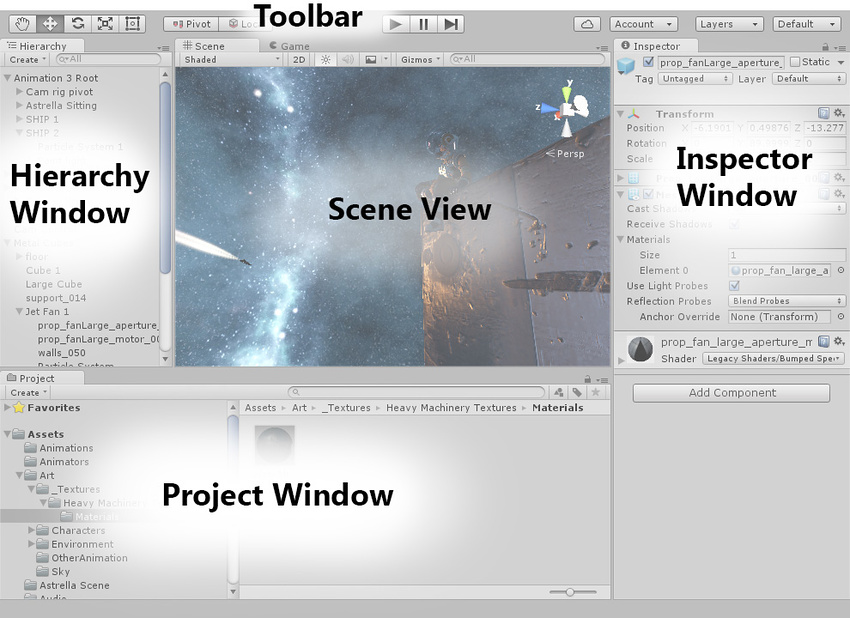
\includegraphics[width=0.9\textwidth]{images/Editor-Breakdown.jpg}
    \caption{Графический интерфейс редактора Unity.%
    \cite{DocUnity}}
    \label{figure:UnityInterface}
\end{figure}

Unity имеет встроенные модули для работы с
графикой, пользовательским вводом, физикой,
пользовательским интерфейсом и сетевым взаимодействием.
Компонентная архитектура фреймворка позволяет
легко расширять уже существующую функциональность.

Основное направление использования Unity -- это разработка игр,
тем не менее Unity также успешно применяется в киноиндустрии,\cite{UnityInFilmmaking}
архитектуре, автомобилестроении,\cite{UnityInAutomotive}
разработке виртуальных тренажеров, а также в
обучении искусственного интеллекта.\cite{UnityInAI}

\paragraph{C\#}
C\#~--~высокоуровневый мультипарадигменный язык общего назначения,
разработанный компанией Microsoft в 1998-2001 годах
в рамках платформы .NET Framework.
C\# относится к семье языков с C-подобным синтаксисом и
используется для написания веб-приложений,
приложений для персональных компьютеров и мобильных устройств.
\cite{DocCSharp}
C\# является основным скриптовым языком фреймворка Unity,
тем самым он используется для написания всей
клиентской и серверной логики разрабатываемого прототипа.

\paragraph{SteamVR}
SteamVR~--~это инструмент, унифицирующий работу с различными
устройствами виртуальной реальности,
разработанный компанией Valve~Corporation.%
\cite{SteamVR}
SteamVR обладает плагинами для фреймворков Unity и Unreal~Engine,
что позволяет интегрировать его в разрабатываемый прототип. 

\paragraph{HTC~Vive}

HTC~Vive~--~это шлем виртуальной реальности,
разрабатываемый компаниями HTC и Valve~Corporation.%
\cite{HTCVive}
HTC~Vive используется во время тестирования прототипа.

\paragraph{3ds~Max}

3ds~Max~--~профессиональное программное обеспечение для 3D-моделирования,
разрабатываемое компанией Autodesk.
3ds~Max является расширяемым инструментом,
что позволяет автоматизировать часть процессов
через создание дополнительных плагинов.%
\cite{Doc3DSMAX}
3ds~Max используется в процессе преобразования информационной модели
из rvt-формата в формат fbx.
